\documentclass{article}
\usepackage{graphicx}
\usepackage{color}
\color{black}

% Margin on left side of page is 1.0 inches plus \oddsidemargin.
\oddsidemargin  -0.75in
\evensidemargin  0pt
% Margin on top also appears to be 1.0 inches plus \topmargin (not checked).
\topmargin -0.5in
\headheight 0.0in
\headsep 0.0in
\marginparwidth 0pt
\marginparsep 0pt
\textwidth   7.5in
\textheight  10.6in

\title{CSE166 - Image Processing - Homework 6}
\author{Nitay Joffe}
\date{November 21, 2006}

\begin{document}
\maketitle

\noindent
{\bf Written exercises}
\begin{enumerate}
  \item Restate the definition (e.g., from your old linear algebra
  textbook) of {\em positive semidefinite}.  Prove that the second
  moment matrix (as defined in class) is positive semidefinite.\\
  \linebreak\linebreak
  A positive semidefinite matrix is a Hermitian matrix whose eigenvalues are
  all nonnegative. A Hermitian matrix is one where $A$ = $A^H$, or
  $a_{ij} = \overline{a}_{ji}$. The second moment matrix has the form
  $\left[\begin{array}{cc}
           a & b\\
           b & c
         \end{array}\right]$. Since a,b and c are all
  real, and it is diagonal, the second moment matrix is clearly Hermitian.\\

  \item The {\em homogeneous coordinates} for a point with cartesian
  coordinates $(x,y)$ are obtained by adding a third coordinate of 1 to
  the cartesian coordinates, i.e.\ $(x,y)$ becomes $(x,y,1)$.  Show how
  one can solve for the affine parameters all at once (instead of
  separating out the translation part as we did in class) using
  homogeneous coordinates and the following parameter matrix (in place
  of $A$ and $\bf t$):
  \[
  B=\left[
  \begin{array}{ccc}
  a_{11}&a_{12}&t_1\\
  a_{21}&a_{22}&t_2\\
  0&0&1
  \end{array}
  \right]
  \]
  \linebreak\linebreak
  $$\left[\begin{array}{c}x'\\y'\end{array}\right]
    = \left[\begin{array}{cc}a_{11}&a_{12}\\a_{21}&a_{22}\end{array}\right]
    \left[\begin{array}{c}x\\y\end{array}\right]
    + \left[\begin{array}{c}t_1\\t_2\end{array}\right]$$
  $$\left[\begin{array}{c}x'\\y'\\1\end{array}\right]
    = \left[\begin{array}{ccc}a_{11}&a_{12}&t_1\\
                              a_{21}&a_{22}&t_2\\
                              0&0&1\end{array}\right]
    \left[\begin{array}{c}x\\y\\1\end{array}\right]$$\\
\end{enumerate}
{\bf Matlab exercises}
\begin{enumerate}
  \item
  \begin{enumerate}
    \item[(b)]
    \begin{verbatim}
t =

    1.9089
   -1.6116


A =

    0.9194   -0.4889
    0.4765    1.0201
    \end{verbatim}
    \item[(c)]
    \begin{verbatim}
distance_before_alignment =

    5.2030


distance_after_alignment =

    0.8214
    \end{verbatim}
  \end{enumerate}
\end{enumerate}
\pagebreak
\begin{verbatim}
% Author: <njoffe@ucsd.edu> Nitay Joffe
% Date: 11/21/2006
% Class: CSE 166 - Image Processing
% Homework: 6
% Problem: 1 - Estimating Affine Transformations
clear;

% (a) Plot the two pointsets on the same set of axes. Use the 'x-'
%     pointmarker/linetype for the first set and 'o-' for the second.
set_1_x = [1.8158,1.8626,3.4883,1.8860,1.8860,3.5234];
set_1_y = [4.0673,2.7924,2.6170,2.4181,1.1667,1.2135];
set_1 = [set_1_x;
         set_1_y];

set_2_x = [1.5468,2.2251,3.9327,2.4942,3.1140,4.4591];
set_2_y = [3.5760,2.0322,2.6170,1.5877,0.5585,1.4123];
set_2 = [set_2_x;
         set_2_y];

% (b) Solve for the least-squares affine transform (consisting of a 2 x 2 matrix
%     A and a 2 x 1 translation vector t) that maps the first pointset onto the
%     second. Display the values you obtain for A and t.
set_1_homogeneous = [set_1;
                     ones(1,size(set_1,2));];
set_2_homogeneous = [set_2;
                     ones(1,size(set_2,2));];
A = set_2_homogeneous / set_1_homogeneous;
t_x = A(1,3);
t_y = A(2,3);
t = [t_x;
     t_y]
A = A(1:2,1:2)

% (c) Use the estimated affine transform to align the two pointsets, and make a
%     plot to show the alignment. Compute and display the sum of the squared
%     Euclidean distances between the corresponding point pairs before and
%     after alignment.
set_1_projected = A * set_1;
set_1_projected_x = set_1_projected(1,:) + t_x;
set_1_projected_y = set_1_projected(2,:) + t_y;

distance_before_alignment = sum(sqrt((set_1_x-set_2_x).^2+(set_1_y-set_2_y).^2))
distance_after_alignment = sum(sqrt((set_1_projected_x-set_2_x).^2+(set_1_projected_y-set_2_y).^2))


figure;
subplot(1,2,1);
plot(set_1_x,set_1_y,'x-');
hold;
plot(set_2_x,set_2_y,'o-');
title('x = pointset 1, o = pointset 2');
subplot(1,2,2);
plot(set_2_x,set_2_y,'x-');
hold;
plot(set_1_projected_x,set_1_projected_y,'o-');
title('x = pointset 2, o = pointset 1 projected');
\end{verbatim}
\pagebreak
\begin{verbatim}
% Author: <njoffe@ucsd.edu> Nitay Joffe
% Date: 11/21/2006
% Class: CSE 166 - Image Processing
% Homework: 6
% Problem: 2 - Interest Point Detection
% Part: a
clear;

% (a) Compute the eigenvalues (\lambda_{max},\lambda_{min}) of the Forstner
%     interest operator for the checker-board image in the figure for GW Problem
%     10.18(right). Use a window size of 3 x 3. On top of the original
%     checkerboard image, plot the coordinates (use the '.' pointmarker) of all
%     pixels for which \lambda_{min} > \tau , with \tau set to 80% of the
%     maximum value of \lambda_{min} over the whole image. The resulting
%     coordinates should fall on or near the corners of the squares in the image.
I = double(imread('Prob10.18(right).jpg'));
[gradient_x,gradient_y] = gradient(I);
gradient_x_squared = gradient_x.*gradient_x;
gradient_y_squared = gradient_y.*gradient_y;
gradient_x_times_y = gradient_x.*gradient_y;
window_1d = [1 1 1];
sum_x_squared_window = conv2(window_1d,window_1d,gradient_x_squared,'same');
sum_y_squared_window = conv2(window_1d,window_1d,gradient_y_squared,'same');
sum_x_times_y_window = conv2(window_1d,window_1d,gradient_x_times_y,'same');

[rows,columns] = size(sum_x_times_y_window);
maximum_eigenvalue_small = 0;
eigenvalues_small = [];
for i=1:rows
  for j=1:columns
    C = [sum_x_squared_window(i,j),sum_x_times_y_window(i,j);
         sum_x_times_y_window(i,j),sum_y_squared_window(i,j)];
    small_eigenvalue = min(eig(C));
    eigenvalues_small(i,j) = small_eigenvalue;
    if (small_eigenvalue > maximum_eigenvalue_small)
      maximum_eigenvalue_small = small_eigenvalue;
    end
  end
end
tau_fraction_of_max_eigenvalue_small = 0.8;
tau = tau_fraction_of_max_eigenvalue_small * maximum_eigenvalue_small;
corners = [];
for i=1:rows
  for j=1:columns
    if (eigenvalues_small(i,j) > tau)
      corners(:,end+1) = [i;j];
    end
  end
end
corners_x = corners(1,:);
corners_y = corners(2,:);


figure;
imshow(I);
hold;
plot(corners_x,corners_y,'.');
title('Checkerboard with interesting points');
\end{verbatim}
\pagebreak
\begin{verbatim}
% Author: <njoffe@ucsd.edu> Nitay Joffe
% Date: 11/21/2006
% Class: CSE 166 - Image Processing
% Homework: 6
% Problem: 2 - Interest Point Detection
% Part: b
clear;

% (b) Repeat the above steps for the fingerprint image in GW Figure 10.29(a);
%     this time set \tau to 20% of the maximum value of \lambda_{min} over the
%     whole image. The resulting coordinates should fall on or near the minutia
%     points of the fingerprint, but due to noise, there will also be many
%     spurious responses. As a final step, compute \phi, the angle of the
%     principal eigenvector for each pixel, and display it as an image.
I = imread('Fig10.29(a).jpg');
[gradient_x,gradient_y] = gradient(double(I));
gradient_x_squared = gradient_x.*gradient_x;
gradient_y_squared = gradient_y.*gradient_y;
gradient_x_times_y = gradient_x.*gradient_y;
window_1d = [1 1 1];
sum_x_squared_window = conv2(window_1d,window_1d,gradient_x_squared,'same');
sum_y_squared_window = conv2(window_1d,window_1d,gradient_y_squared,'same');
sum_x_times_y_window = conv2(window_1d,window_1d,gradient_x_times_y,'same');

[rows,columns] = size(sum_x_times_y_window);
maximum_eigenvalue_small = 0;
eigenvalues_small = [];
phi = [];
for i=1:rows
  for j=1:columns
    C = [sum_x_squared_window(i,j),sum_x_times_y_window(i,j);
         sum_x_times_y_window(i,j),sum_y_squared_window(i,j)];
    phi(i,j) = 0.5*atan2(2*sum_x_times_y_window(i,j),sum_x_squared_window(i,j)-sum_y_squared_window(i,j));
    small_eigenvalue = min(eig(C));
    eigenvalues_small(i,j) = small_eigenvalue;
    if (small_eigenvalue > maximum_eigenvalue_small)
      maximum_eigenvalue_small = small_eigenvalue;
    end
  end
end
tau_fraction_of_max_eigenvalue_small = 0.2;
tau = tau_fraction_of_max_eigenvalue_small * maximum_eigenvalue_small;
corners = [];
for i=1:rows
  for j=1:columns
    if (eigenvalues_small(i,j) > tau)
      corners(:,end+1) = [i;j];
    end
  end
end
corners_x = corners(1,:);
corners_y = corners(2,:);


figure;
imshow(I);
hold;
plot(corners_x,corners_y,'.');
title('Fingerprint with interesting points');
figure;
imshow(phi);
title('phi');
\end{verbatim}
\pagebreak
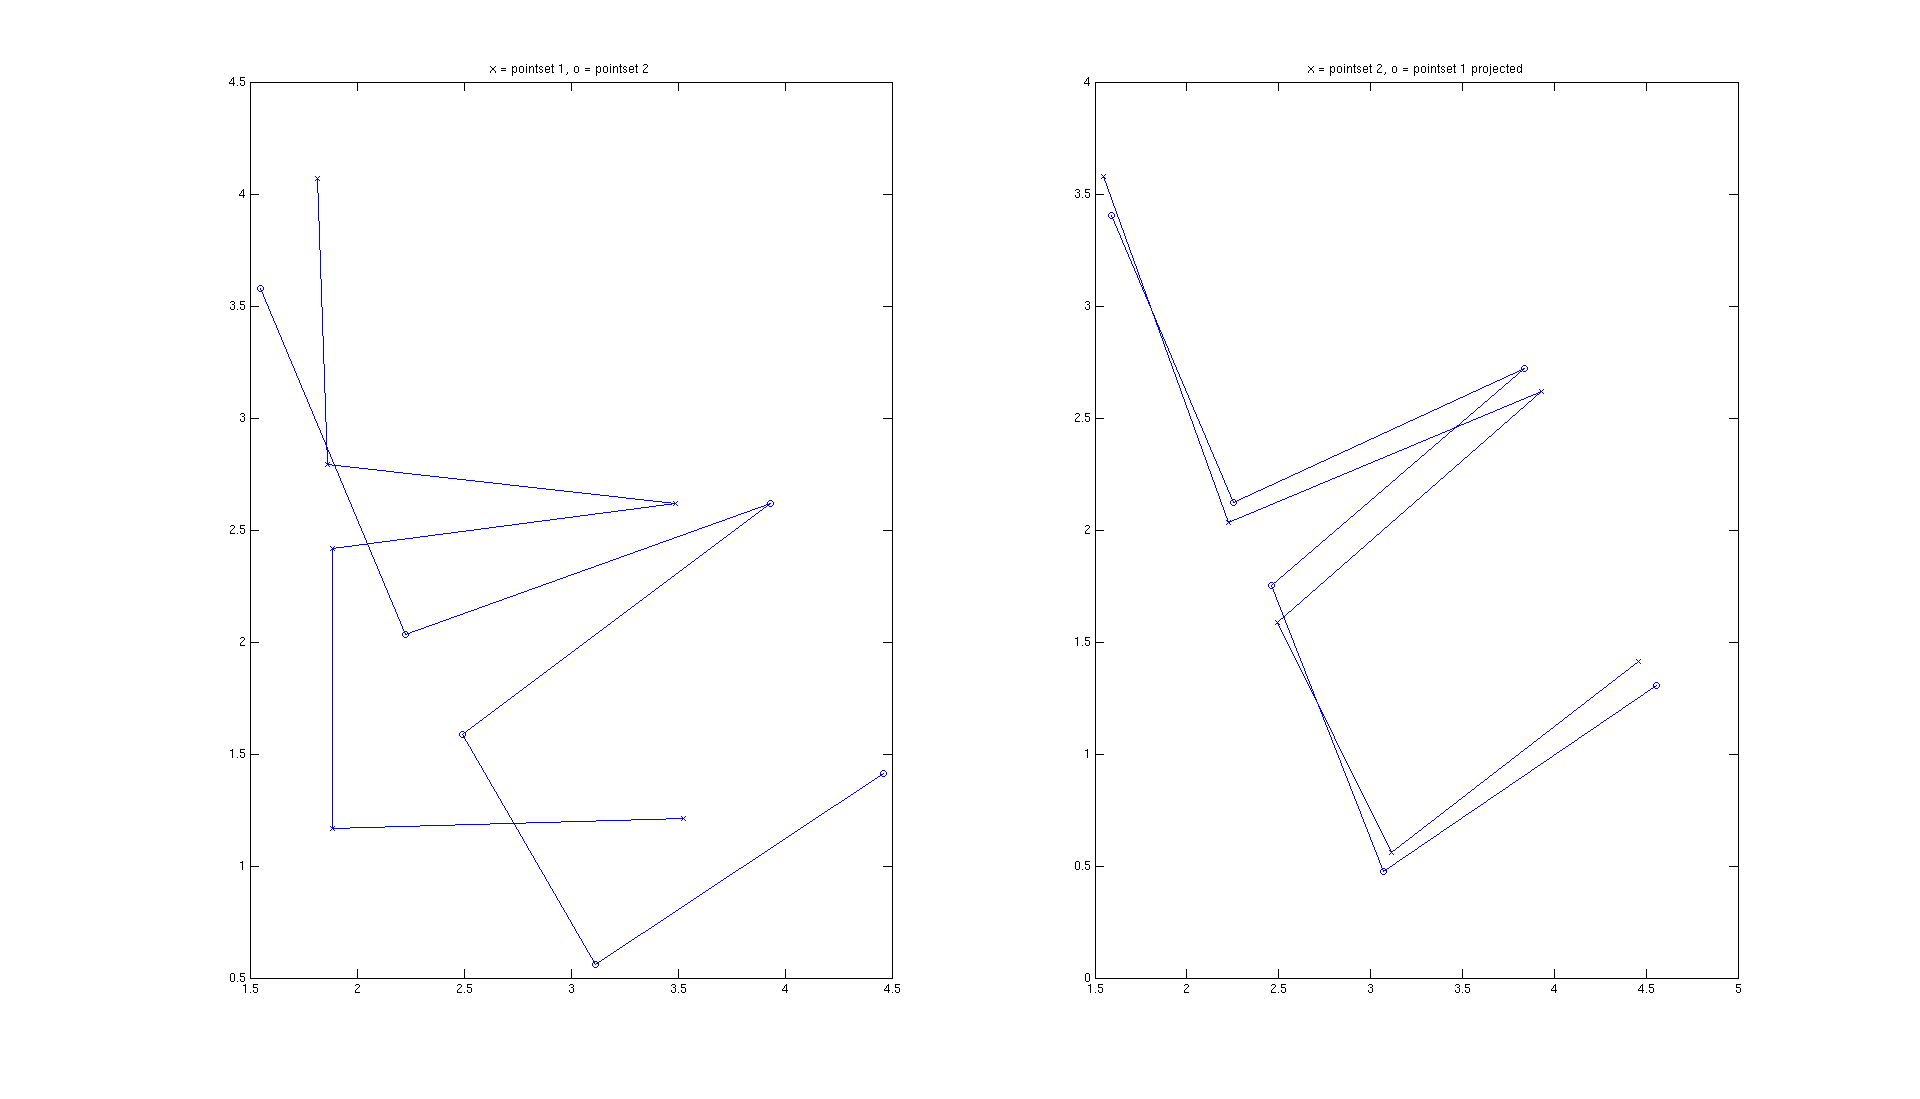
\includegraphics [width=8in]{1.png}
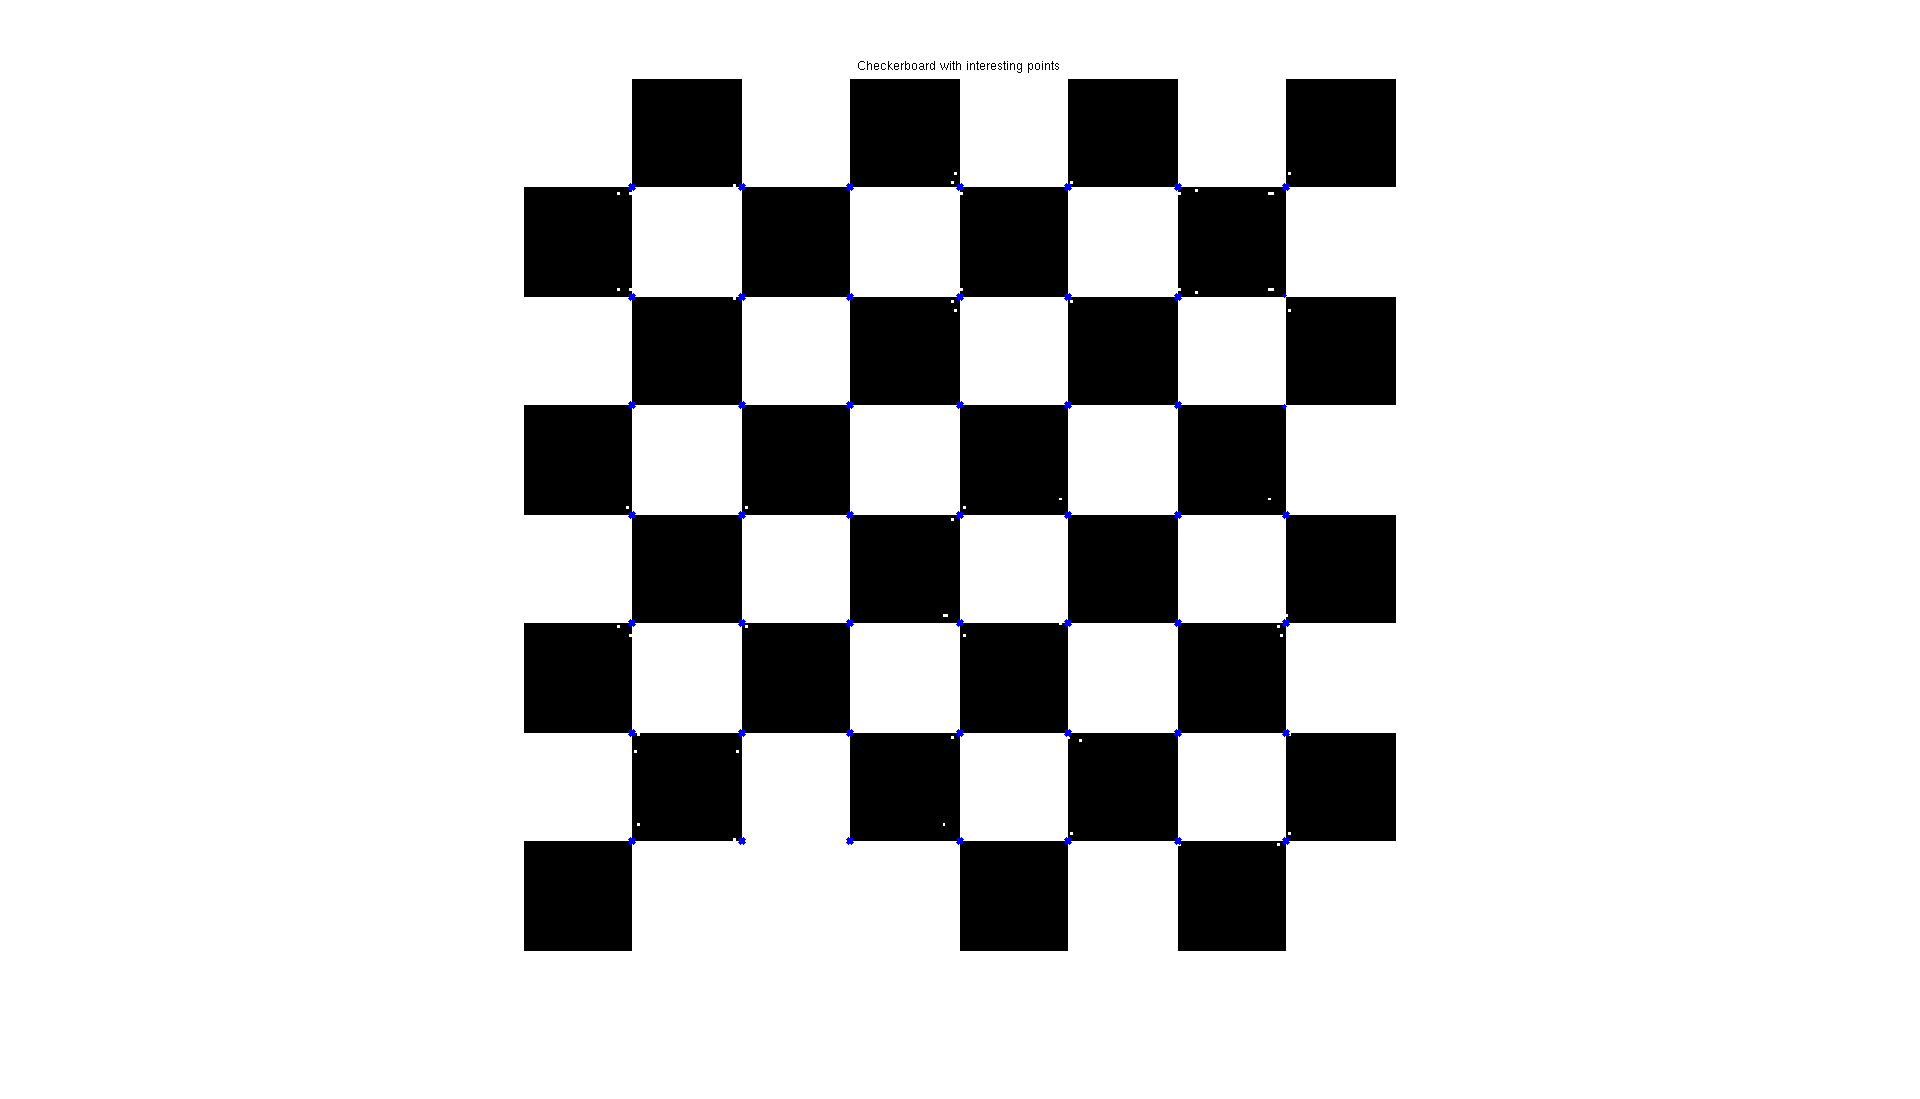
\includegraphics [width=9in]{2a.png}
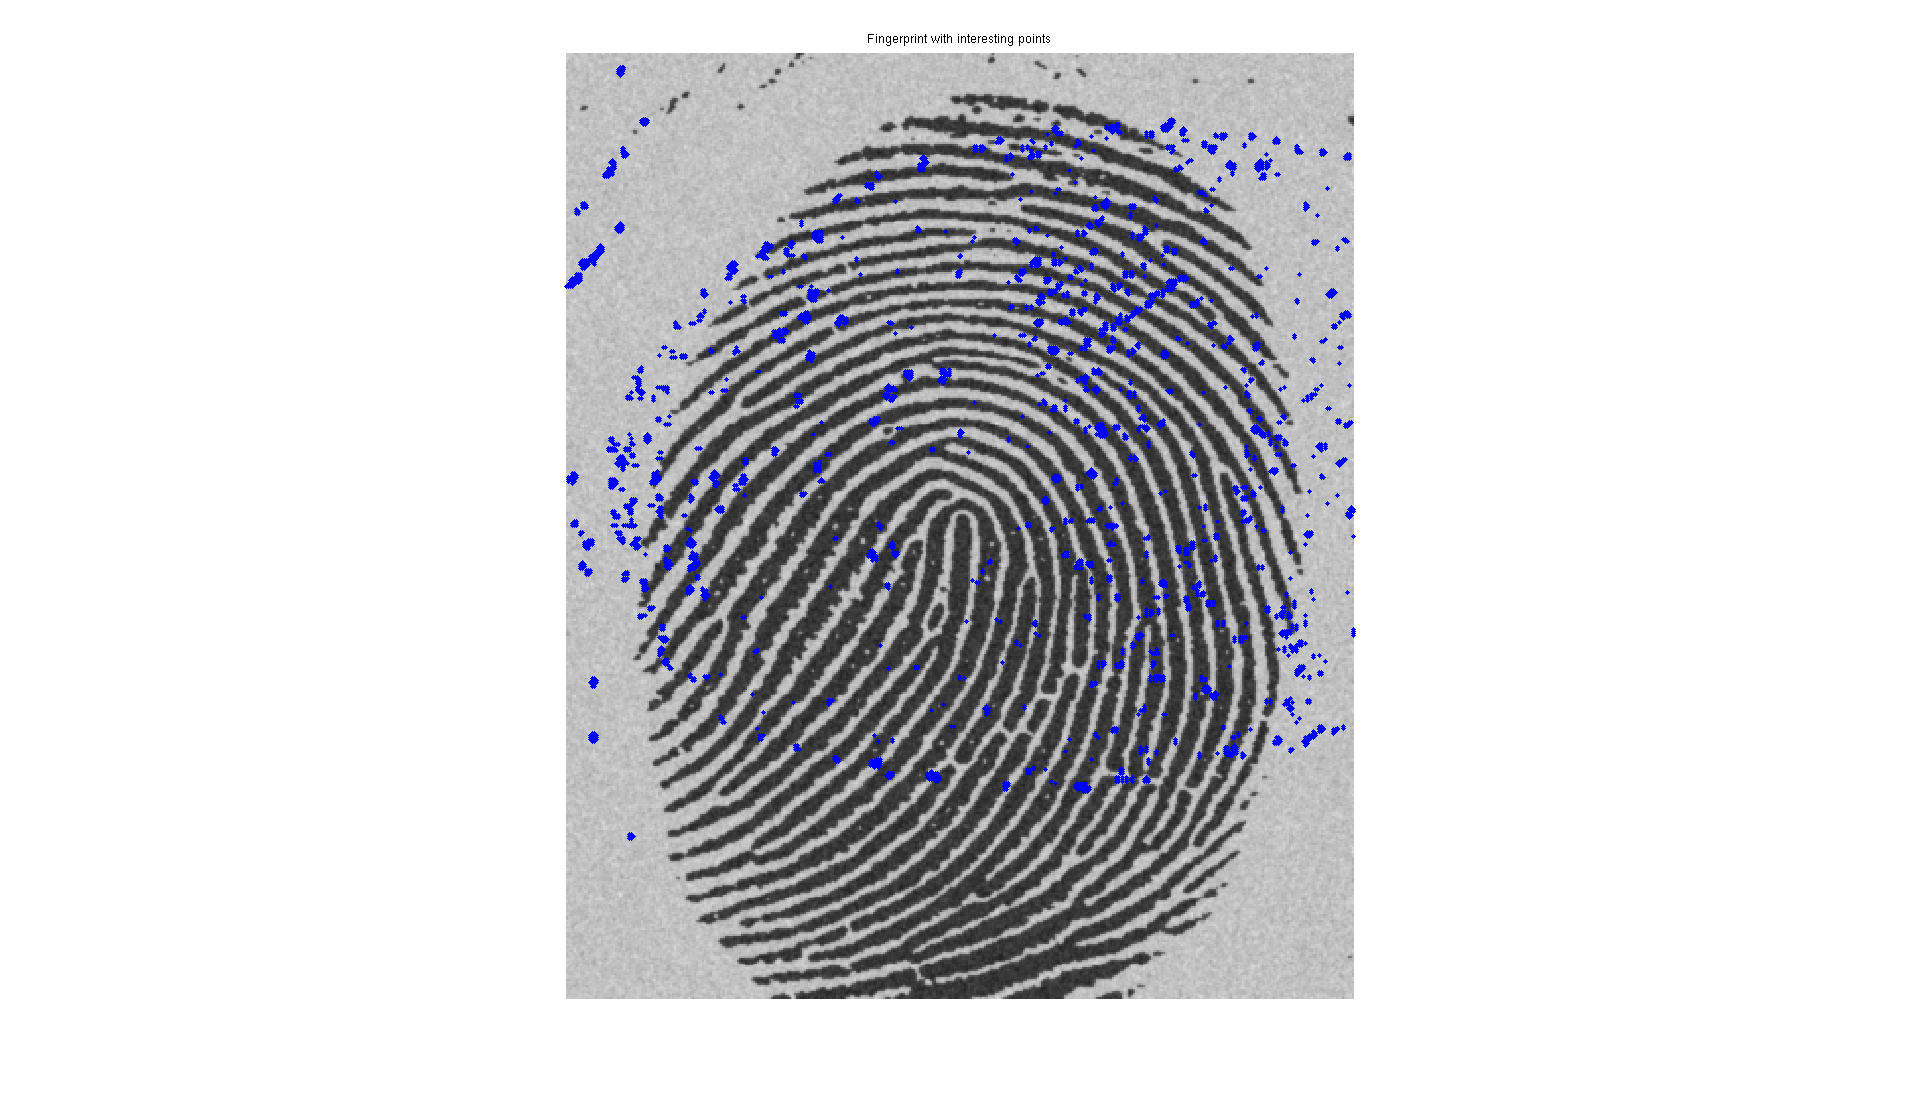
\includegraphics [width=9in]{2b_1.png}
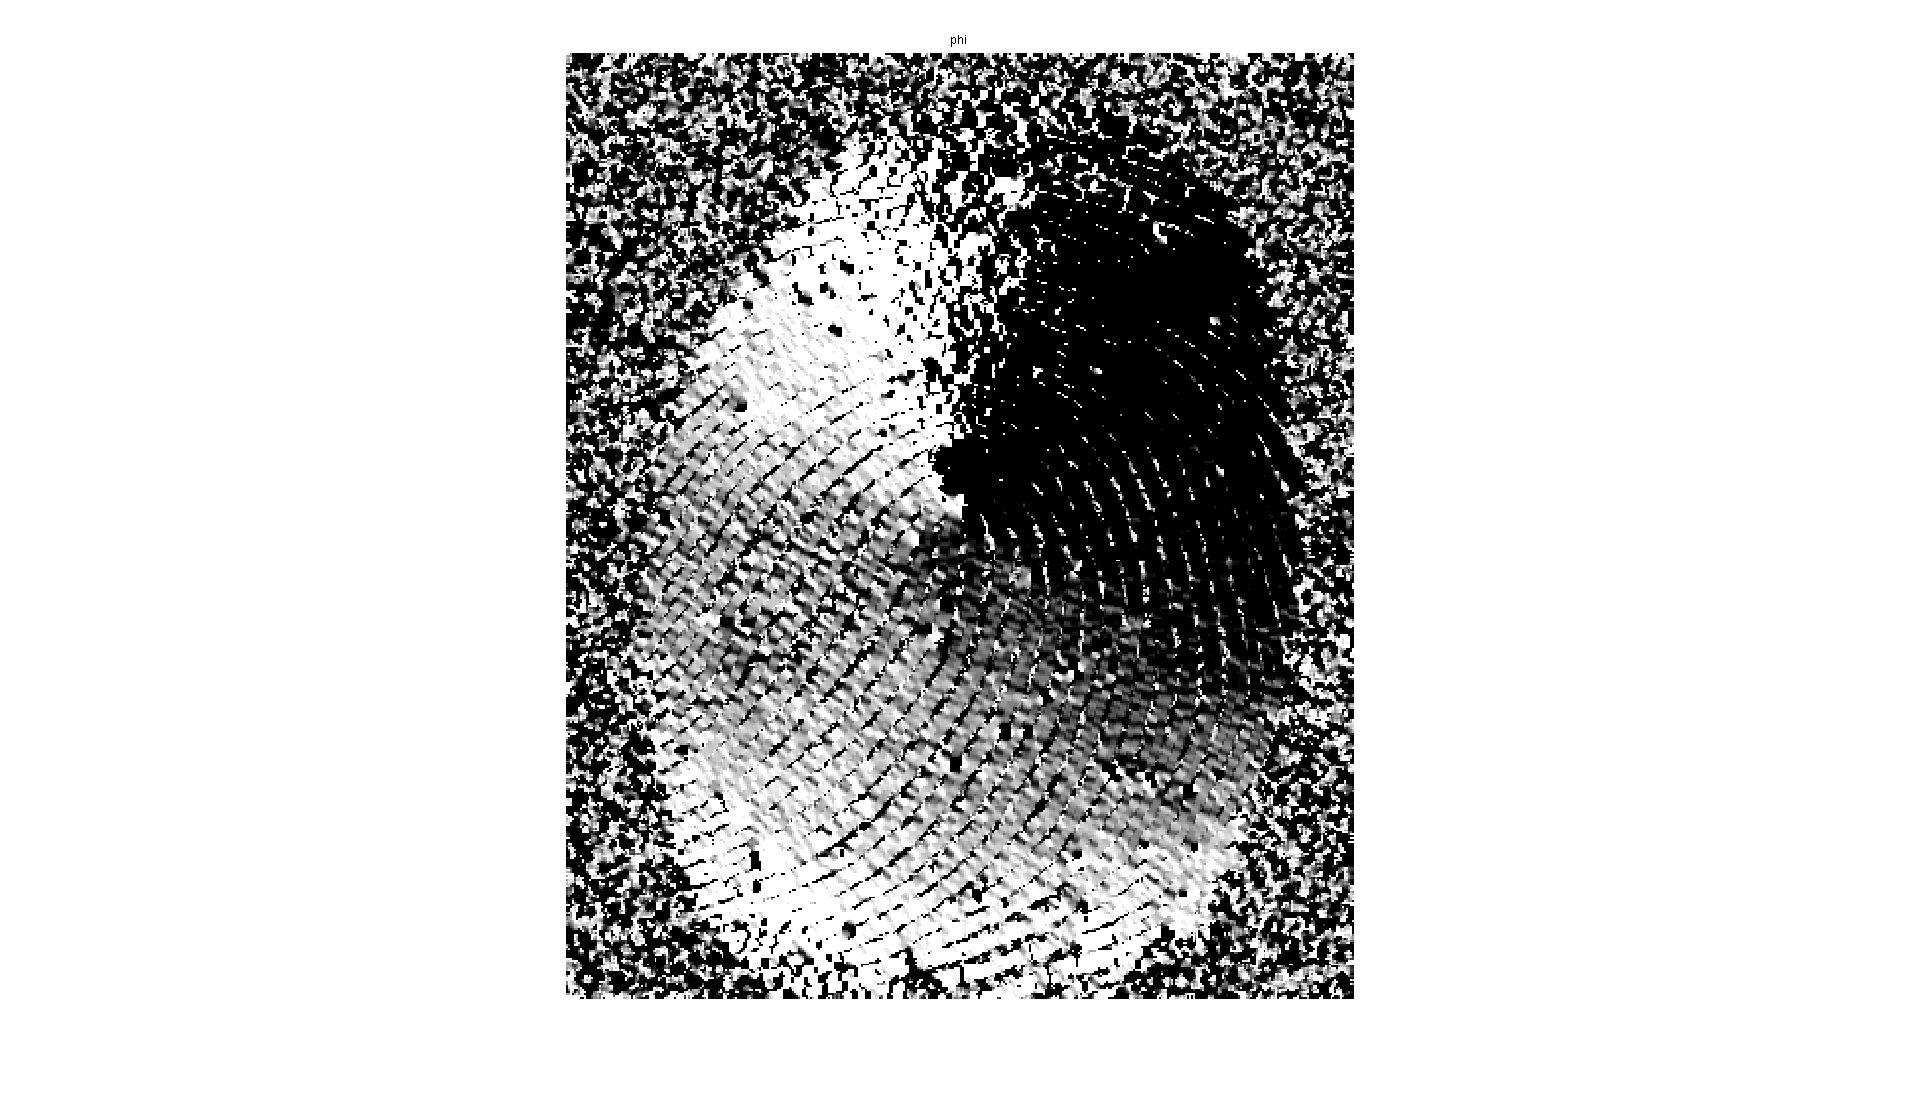
\includegraphics [width=9in]{2b_2.png}
\end{document}
